\section{Results}

\subsection{Exploratory analyses}
In order to obtain an overview of the dataset structure, Principal Component Analysis (PCA) was performed and chromosomal CNAs were visualized, ordered by clinical subgroup. However, PCA results were not suitable to detect any separation of subgroups once projected on the first two Principal Components (combined explained variance of only 22.21\%). Moreover, visualization of chromosomal CNAs failed to point out obvious discriminatory features for subgroups. Altogether, these findings indicated that further feature selection was needed before classification model training.

\subsection{Benchmark of classifiers}
    \subsubsection{Nested cross-validation}
        We employed a nested 10-fold stratified cross-validation scheme, with inner loop for feature selection / hyperparameter selection and outer loop for model training, both loops split the samples to 70\% training and 30\% testing (see Methods for full details).
        
        Initially, Pearson's chi-squared test for differences between clinical subgroups was conducted per feature, with a Bonferroni-adjusted threshold P-value of $0.05 * 2,834$. However, still at several hundred significant features for most models, we tested more stringent P-values (0.01, 0.001). 
        Initially, Pearson's chi-squared test for differences between clinical subgroups was conducted per feature. We performed a test for the significance threshold by nested CV with a 1-fold outer and 10-fold inner loop to check for the effect on the accuracy of the training as well as the validation and the amount of selected features. It was observed that the amount of features selected decreases upon lowering the significance threshold for all classifiers (NSC: 586, 195, 36; KNN: 421, 206, 28; NNet: 421, 207, 36). For NSC, upon lowering the significance threshold (0.05, 0.01, 0.001) a relatively stable training accuracy (0.70, 0.69, 0.69) and increasing validation accuracy (0.54, 0.64, 0.68) was observed. For KNN, an increasing trend was observed for both the training accuracy (0.58, 0.62, 0.67) and the validation accuracy (0.57, 0.57, 0.64). For Neural Network, the training accuracy remained relatively stable (0.76, 0.77, 0.75) whereas the validation accuracy fluctuated (0.75, 0.61, 0.71). Considering all classifiers, the significance threshold of 0.001 was selected for feature selection with Pearson's Chi-squared test.
    
    \subsubsection{Performance of classifiers}
        We benchmarked neural networks, K-nearest neighbors (KNN) and nearest shrunken centroids (NSC) as classifiers with chi-squared test and Boruta (\citealp{Kursa2010}) as feature selection methods, using the accuracy as performance metric. This revealed that a neural network (hyperparameters: decay = 0.01, size = 5) with 38 Boruta-selected features performed best at classifying clinical subgroups with an accuracy of 0.895. A comprehensive overview of all models is displayed in Table~1\vphantom{\ref{Tab:01}}.
        
        Overall, the neural networks performed better than KNN models, which subsequently outperformed all NSC models. Chi-squared feature selection in neural network and KNN models had in fact identical accuracy and other performance metrics. Boruta outperformed chi-squared as feature selection method for both neural network and KNN models, albeit with a difference of only 0.055 on average, while Boruta failed to outperform the chi-squared model of NSC. One consistency in all neural network and KNN models were perfect HER2+ specific performance metrics. Finally, while the F1-score was consistently lower in the triple negative subgroup of neural network and KNN models, the best-performing model did reach a F1-score of 0.833 for this apparently more challenging classification subject.
    
    \begin{table}[!t]
        \processtable{Metrics of (subgroup-specific) performance for cross-validated models\label{Tab:01}} {\begin{tabular}{@{}lllllll@{}}
        \toprule Model & Feature selection & Accuracy & Subgroup & Specificity & Sensitivity & F1 \\
        \midrule
        NN & Chi-squared  & 0.821  & HER2+ & 1     & 1     & 1\\
           &              &       & HR+   & 0.882 & 0.727 & 0.762\\
           &              &       & TN    & 0.850 & 0.750 & 0.706\\
        NN & Boruta       & 0.895 & HER2+ & 1     & 1     & 1\\
           &              &       & HR+   & 0.917 & 0.857 & 0.857\\
           &              &       & TN    & 0.923 & 0.833 & 0.833\\
        KNN & Chi-squared & 0.821 & HER2+ & 1     & 1     & 1\\
           &              &       & HR+   & 0.882 & 0.727 & 0.762\\
           &              &       & TN    & 0.850 & 0.750 & 0.706\\
        KNN & Boruta      & 0.857 & HER2+ & 1     & 1     & 1\\
           &              &       & HR+   & 0.889 & 0.8   & 0.8\\
           &              &       & TN    & 0.894 & 0.778 & 0.778\\
        NSC & Chi-squared & 0.786 & HER2+ & 0.950 & 1     & 0.941\\
           &              &       & HR+   & 0.810 & 0.857 & 0.706\\
           &              &       & TN    & 0.933 & 0.615 & 0.727\\
        NSC & Boruta      & 0.750 & HER2+ & 1     & 1     & 1\\
           &              &       & HR+   & 0.789 & 0.667 & 0.632\\
           &              &       & TN    & 0.833 & 0.6   & 0.632\\
        \botrule
        \end{tabular}}{NN, neural network; KNN, K-nearest neighbors; NSC, nearest shrunken centroids; TN, Triple Negative. \\ Selected models had the highest accuracy score for equivalent models in 10-fold stratified cross-validation.}
    \end{table}

\subsection{Evaluation of best model}
    Based on the promising model accuracy score and subgroup-specific metrics, HER2+ in particular, we set out to further evaluate the model and detect potential flaws.
    
    \subsubsection{Clustering of genomic regions}
        The relationships between the best model features in all samples were assessed with average linkage (UPGMA) clustering of chromosomal aberration values as shown in Figure~2\vphantom{\ref{fig:02}}. This was visualized for the features from the best performing Boruta - neural network model (Figure~2A\vphantom{\ref{fig:02}}) and the features, which were also retrieved with Boruta, overlapping between the best models of all classification algorithms (Figure~2B\vphantom{\ref{fig:02}}).
        Amplification events were overall sparse yet dominated the HER2+ subgroup in a cluster-outgroup region of chromosome 17 (Figure~2A\vphantom{\ref{fig:02}}). Besides single occurrences for chromosomes 1, 16 and 22, most chromosomes with multiple occurrences were directly clustered together (3, 5, 10 and 12). It was in chromosomes 6 and 17 that regions were not all directly linked together. The former appeared to be divided by more chromosomal losses for HR+ samples in certain regions, while the latter included the amplification outgroup for HER2+ and a region with more copy losses for HR+ samples. The amplification outgroup was located on a chromosome 17q12 subregion (feature: 2185, hg18: chr17:35076296-35282086) and included \textit{HER2}/\textit{ERBB2} for which amplification is a hallmark in the HER2+ subgroup (\citealp{Harbeck2019}). All classification algorithms confirmed the amplification outgroup 17q12 to be able to classify HER2+ samples (Figure 2B). For the remainder of the shared features, clustering of the chromosomes occurred in an ordered fashion. Here, it can be observed that chromosomal gains for HR+ occur relatively more often at chromosome 12q21.31 subregion (feature: 1678, chr12:84542006-85443011 \& feature: 1679, chr12:85450052-85962613) and relatively more chromosomal gains occur for TN at chromosome 22q13.2 subregion (feature: 2752, chr22:41307174-41912419).
        
        \begin{figure}[h]%figure2
            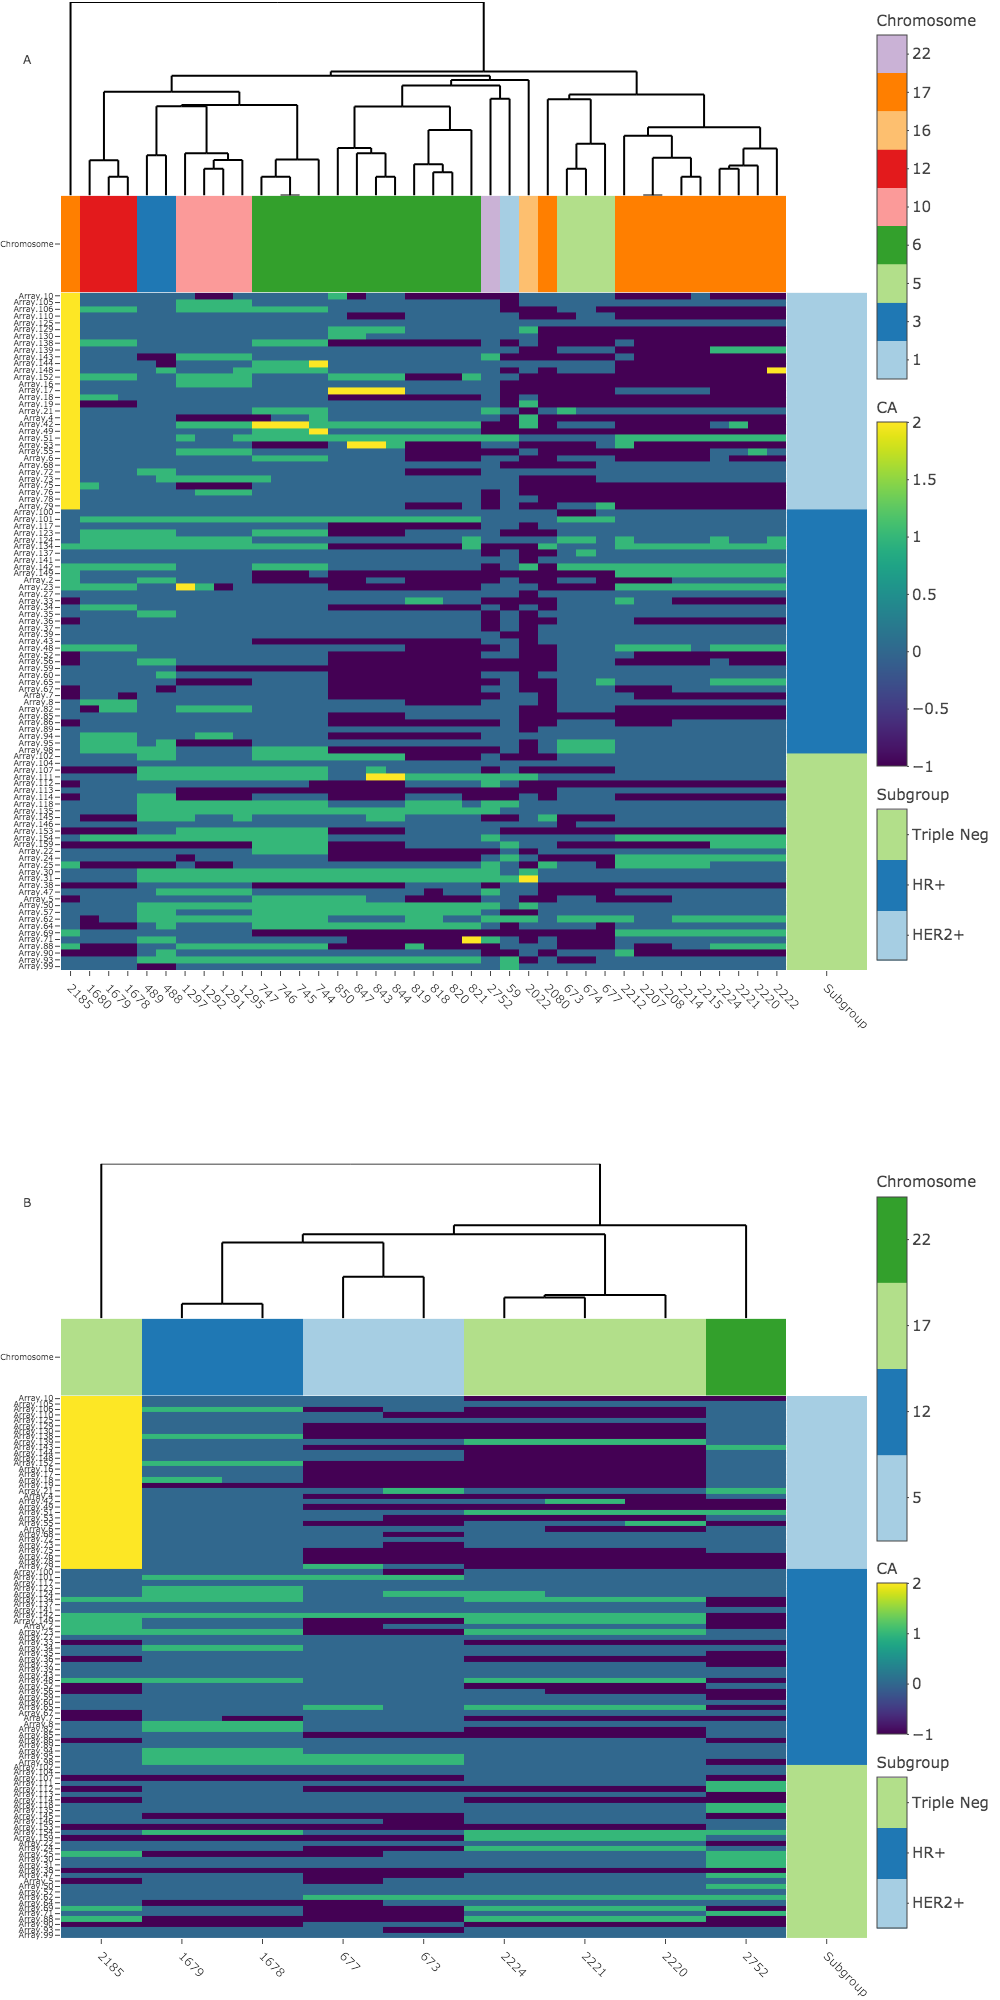
\includegraphics[scale=0.25]{CATS assignment/final-paper/cabios-template/images/figure_2.png}
            \caption{Heatmap of chromosomal abberation patterns of all breast cancer samples A) including only the features from best performing NNet model and B) including features overlapping between the best models of all classification algorithms. The columns depict the chromosomal regions, whereas the rows show all the breast cancer samples, ordered based on subtype ("light blue" equals HER2+, "blue" equals HR+ and "green" equals Triple Negative). The filled tiles represent the different chromosomal aberration states: amplification (+2), gain (+1) and loss (-1). For chromosomal regions, the chromosome number has been shown and have been clustered by hierarchical clustering.}\label{fig:02}
        \end{figure}

    \subsubsection{Permutation analysis}
        To assess the likelihood of obtaining the model's accuracy with these specific features due to chance, we performed a permutation analysis. New feature sets of identical size ($38$ features) were sampled with replacement from the entire feature set, neural networks were trained and tested under identical conditions and hyper parameters, and the accuracy was assessed ($n=1000$). None of the permuted models achieved a similar or higher accuracy than the original model, thus a P-value of $P \approx 0.001$ was assigned to the original model (Figure~2\vphantom{\ref{fig:02}}). These results strongly indicate that the model accuracy can not be attributed to random effects.

    \subsubsection{Identification of genes and biomarkers}
        We investigated the specific genomic regions that served as model features in the best-performing neural network to find biological factors that underpin the model. To accomplish this, genes that were (partially) located within the hg18 reference genome coordinate ranges of model features were obtained and investigated for associations with breast cancer in literature.
        
        The most striking results were the genes identified in the 17q12 subregion, which displayed a distinct amplification in all HER2+ samples in Figure 2B, and included \textit{HER2}/\textit{ERBB2} that is characteristic for HER2+ patients (\citealp{Harbeck2019}). Beyond this single gene, we hypothesized that the 17q12 subregion could be the \textit{HER2} amplicon (\citealp{Sahlberg2013}). We found several genes that provided additional evidence for this hypothesis, including \textit{PNMT}, \textit{GRB7}, \textit{STARD3}, \textit{TCAP} and \textit{PERLD1}, that have been associated with the HER2 amplicon (\citealp{Sahlberg2013}). In addition, all these genes except for \textit{PERLD1} were also found to be important for HER2+ in another breast cancer subtype classification study (\citealp{Pan2019}).
        
        In a subregion of 17q21.31 (feature: 2208, hg18: chr17:38077519-38710043) of the same chromosome we found additional genes with known associations or implications with breast cancer. First and foremost, we found the tumor suppressor and breast cancer hallmark gene \textit{BRCA1} (\citealp{Harbeck2019}). Adjacent to \textit{BRCA1} lies \textit{NBR2} and it has been found to encode for a non-coding RNA with a role in tumor development suppression (\citealp{Xiao2016}) . \textit{AOC3} has previously been implicated in metastatic breast cancer(\citealp{Cha2018}). In another study, \textit{BECN1} was identified as an oncogene with specific involvement in triple negative breast cancer (\citealp{Wu2018}). Finally, the 17q12.31 subregion included \textit{CCR10} which may have a key regulatory role in the cell invasion and migration of breast cancer (\citealp{Lin2017}).
    
        One additional discovery on chromosome 17 was \textit{WNT3}, located in a subregion of 17q21.32 (feature: 2220, hg18: chr17:42161364-42296514), for which previous studies have linked it together with the WNT pathway to HER2-overexpressing cells (\citealp{Wu2017}). Furthermore, \textit{RASSF9} was found in a subregion of chromosome 12q21 (feature: 1678, hg18: chr12:84542006-85443011) and it has been found to be related to breast tumour initiation and propagation in previous studies (\citealp{Li2018}). Finally, we found \textit{CYB5R3} (NADH-Cytochrome B5 Reductase 3) in a subregion of chromosome 22q13 (feature: 2752, hg18: chr22:41307174-41912419) that has been shown to drive metastasis in triple negative (oestrogen receptor negative) breast cancer (\citealp{Lund2015}). Another study (\citealp{Blanke2014}) found that a particular variant of this gene, \textit{I1M+6T}, is more common in breast cancer patients than in controls.
        
        In the end, we investigated the potential of individual model features to serve as biomarker for the clinical subgroups. Earlier on we have shown that a subregion of chromosome 17q12 could completely discriminate HER2+ patients from HR+/triple negative by a distinct amplification pattern (Figure 2) that was reflected by HER2+-specific sensitivity, specificity and F1-scores of 1 for HER2+ in most models, including the best-performing model. Therefore we nominated this feature to serve as biomarker for HER2+ patients, whereas distinct biomarkers for HR+ or triple negative patients were not apparent.
        
        \begin{figure}[]%figure3
            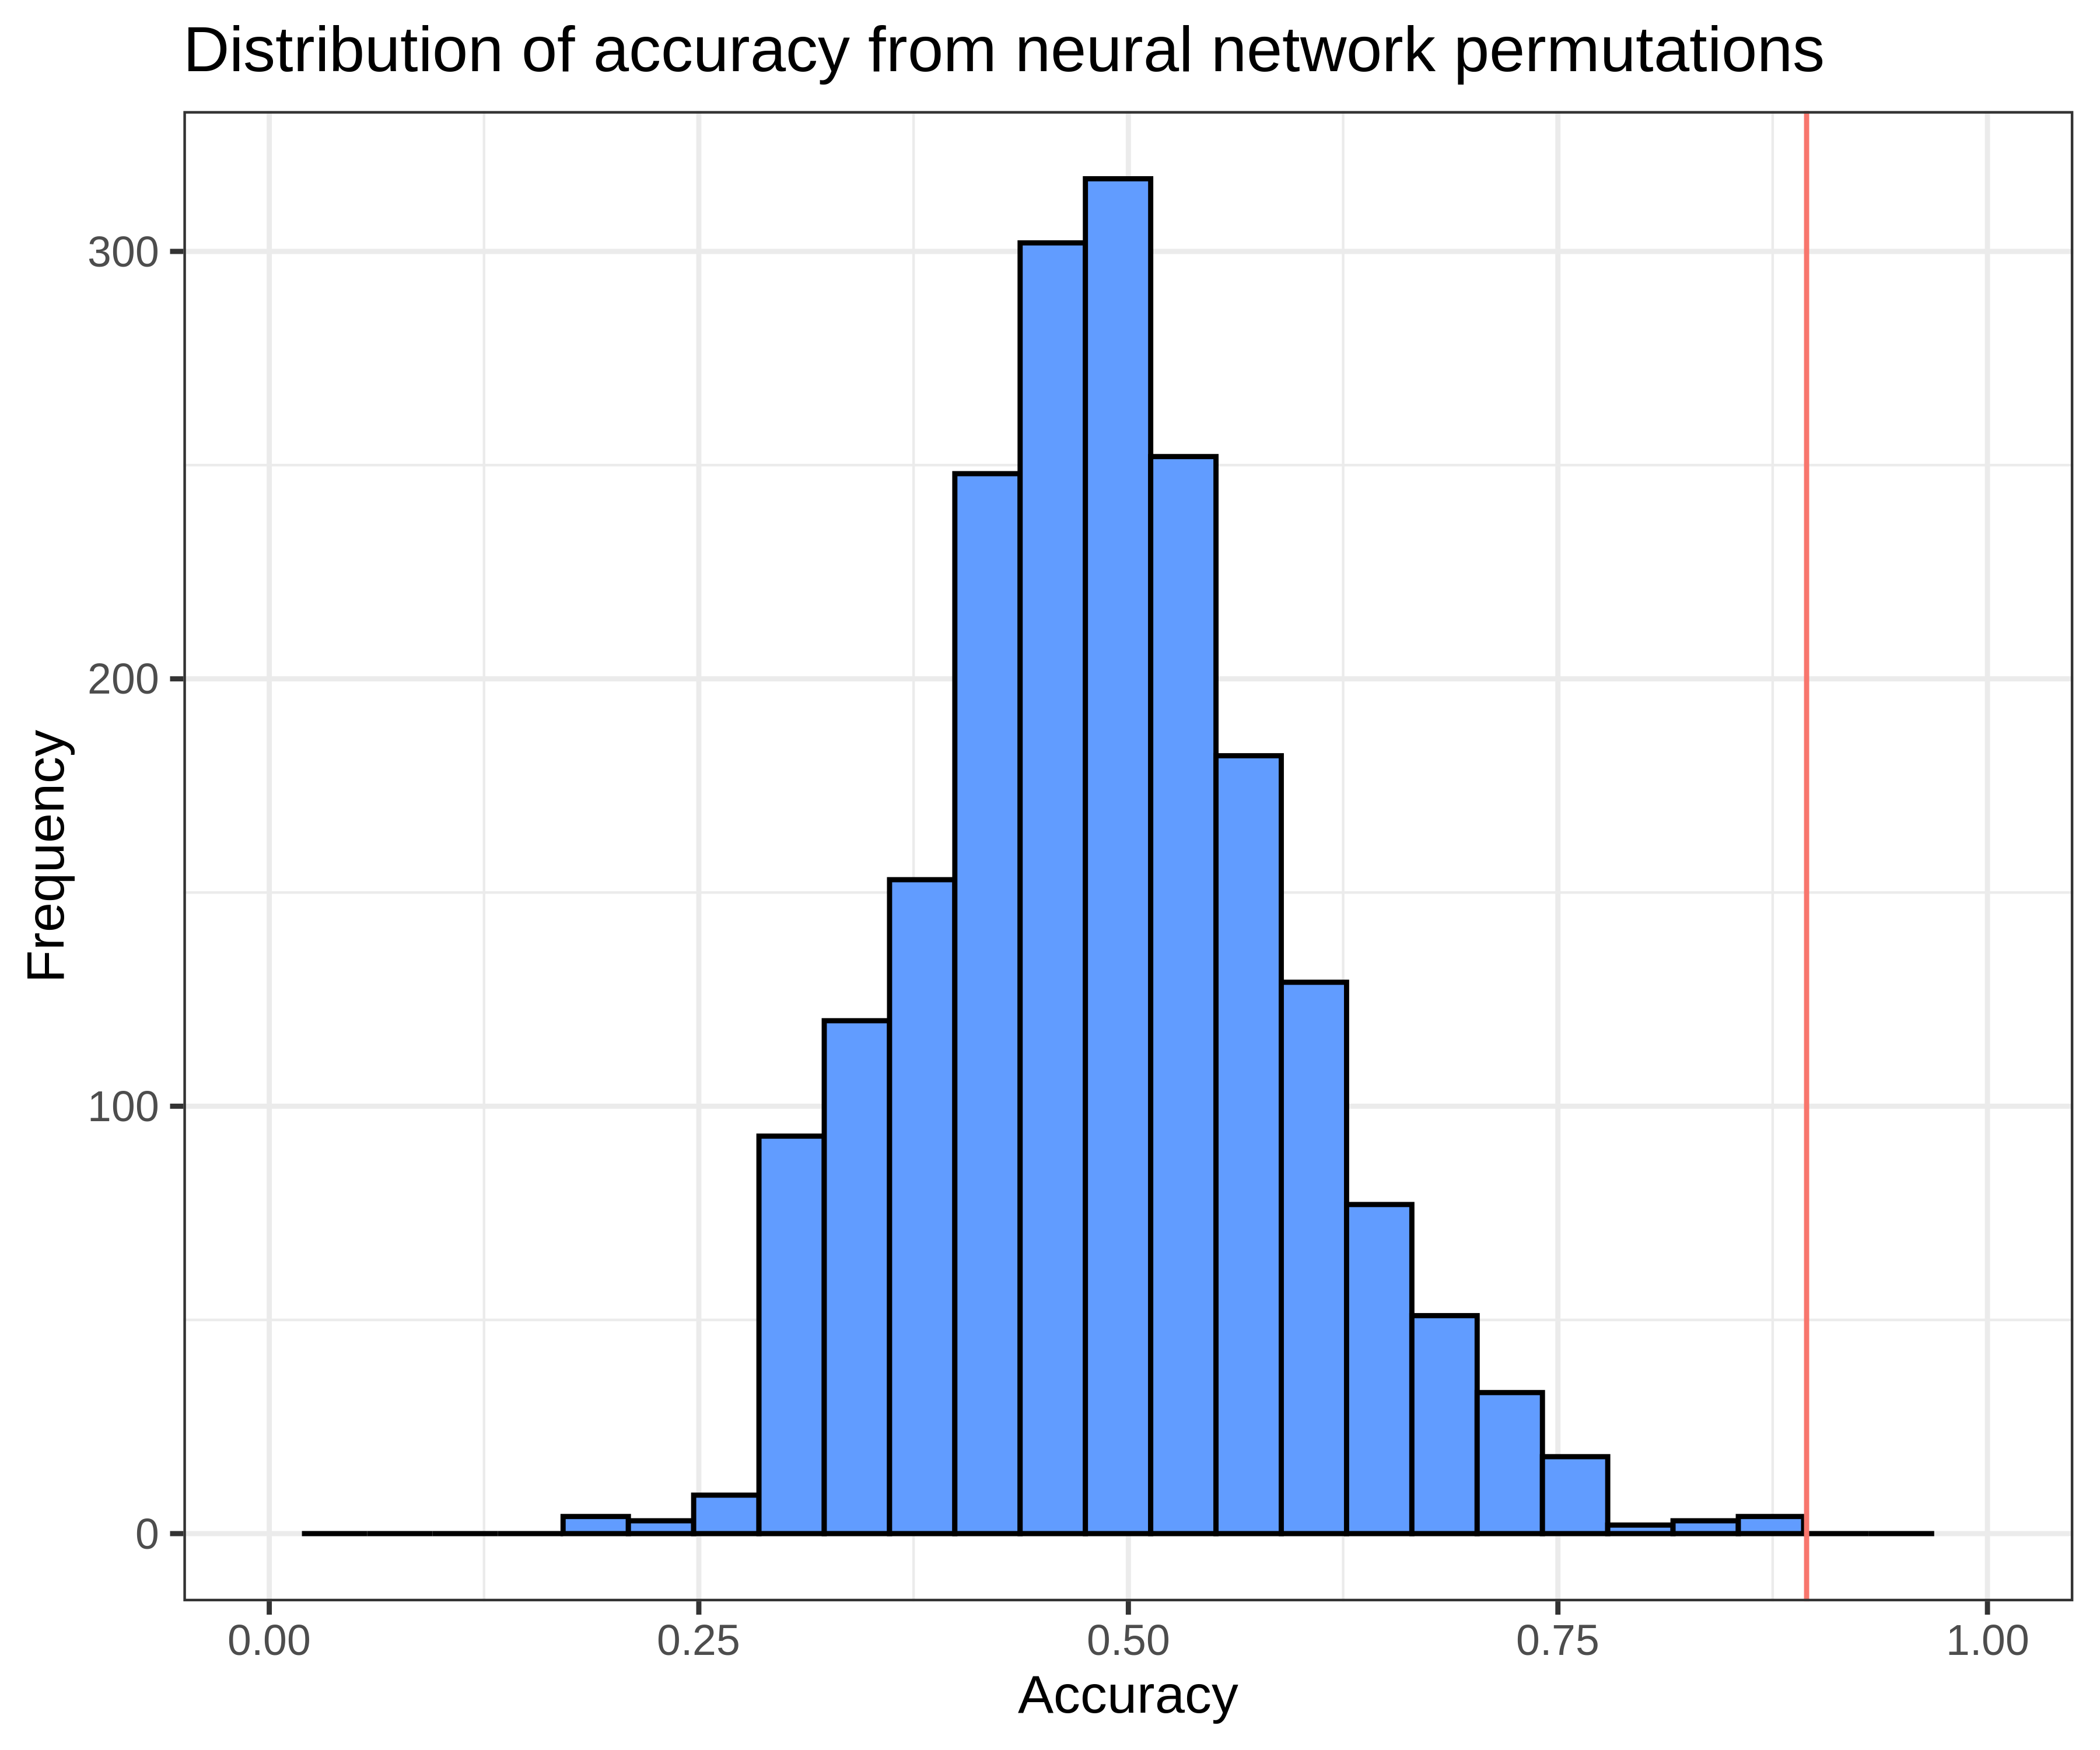
\includegraphics[scale=0.55]{CATS assignment/final-paper/cabios-template/images/figure_3.png}
            \caption{Histogram of accuracy scores for 1000 permuted neural network models (in blue) and the original accuracy (0.895, red line) derived from best-performing neural network model for breast cancer subgroup classification. Accuracy scores of permuted models appear to be normally distributed, none are equal to or are large than the original accuracy score.}\label{fig:03}
        \end{figure}